\documentclass[11pt]{article}

\setlength\textwidth{160mm}
\setlength\textheight{220mm}
\setlength\oddsidemargin{-3mm}
\setlength\headheight{0mm}
\setlength\topmargin{-10mm}

\usepackage{amsfonts}
\usepackage{graphics}
\usepackage{graphicx}

\newtheorem{thm}{Theorem}
\newtheorem{lem}{Lemma}
\newtheorem{cor}{Corollary}
\newtheorem{defn}{Definition}
\newtheorem{fact}{Fact}
\newtheorem{alg}{Algorithm}
\newtheorem{prop}{Proposition}

\begin{document}

\title{A Least Squares Framework for the Maximum Weight Clique Problem
\thanks{Copyright \copyright \ Stanislav Busygin, 2002-2010. All rights reserved.}}

\author{Stanislav Busygin \\
{\tt busygin@gmail.com} \\
{\tt http://www.stasbusygin.org}}

\date{October 14, 2007, updated: May 29, 2010}

\maketitle

% \begin{abstract}
% A simple undirected graph $G(V,E)$, $V=\{1,2, \ldots ,n\}$, with given
% positive vertex weights $w \in \mathbb{R}^n$ is arranged as
% an $(n-1)$-dimensional polyhedron $\Delta^{(w)}_n$ of $n$ vertices in
% $\mathbb{R}^n$. The $i$-th vertex of $\Delta^{(w)}_n$ is located at
% the point $\frac{1}{\sqrt{w_i}} e_i$, where $e_i$ is the $i$-th basis
% vector. We identify a vertex subset of $G(V,E)$ with a face of $\Delta^{(w)}_n$
% formed by this subset. $\Delta^{(w)}_n$ lies within the hyperplane $z^T x = 1$,
% where $z$ is the vector of vertex weight square roots: $z_i = \sqrt{w_i}$.
% An inequality $x^T H x \leq 1$, where $h_{ij} \leq z_i z_j$, holds for any
% point of $\Delta^{(w)}_n$. When $h_{ij} = z_i z_j$ iff $i=j$ or $(i,j) \in E$,
% the equality $x^T H x = 1$ holds iff $x$ is on a clique of $G(V,E)$. This way,
% we define $(n-2)$-dimensional quadratic surfaces characterizing all graph
% cliques. We call such a surface a {\em clique wrapper}.
% 
% The maximum weight clique problem may be formulated as finding a common
% point of $\Delta^{(w)}_n$ and a clique wrapper closest to the origin. This
% corresponds to the following least squares program:
% \[ 1/\omega(G,w) = \min x^T x \]
% \[ \mbox{s.t. } x^T H x = 1, \ z^T x = 1, \ x \geq 0. \]
% When the nonnegativity constraint is relaxed, all stationary points of
% the program can be found via roots of one univariate rational equation.
% If a maximal clique is such that any vertex outside it has the same
% total neighborhood weight in the clique, then the clique may be found via
% a stationary point of the program.
% \end{abstract}

\begin{abstract}
A nonlinear least squares formulation for the maximum weight clique problem
is proposed. When nonnegativity of variables is relaxed, it becomes possible
to enumerate its stationary points assuming the degeneracy did not occur.
It is proved that those stationary points are sufficient to recognize certain
types of maximal cliques.
\end{abstract}

\section{Introduction}
Let $G(V,E)$ be a simple undirected graph, $V=\{1,2, \ldots ,n\}$,
$E \subset V \times V$.
The {\em adjacency matrix\/} of $G$ is a matrix $A_G=(a_{ij})_{n \times n}$,
where $a_{ij} = 1$ if $(i,j) \in E$, and $a_{ij}=0$ if $(i,j) \notin E$.
The set of vertices adjacent to a vertex $i \in V$ will be denoted by
$N(i) = \{j \in V: \ (i,j) \in E\}$ and called the {\em neighborhood} of
the vertex $i$. A {\em clique\/} $Q$ is a subset of $V$ such that any two
vertices of $Q$ are adjacent. The maximum clique problem asks for a clique
of maximum cardinality. This cardinality is called the {\em clique number\/}
of the graph and denoted by $\omega(G)$.

One should not confuse maximum cliques with {\em maximal\/} ones. A clique
$Q$ is called {\em maximal\/} if there is no larger clique in the graph having
$Q$ as its subset. In other words, there is no vertex outside $Q$ connected
with every vertex of $Q$ by an edge.

Next, we associate with each vertex $i \in V$ a positive number $w_i$
called the vertex {\em weight}. This way, along with the adjacency
matrix $A_G$, we consider the vector of vertex weights $w \in \mathbb{R}_+^n$.
We also refer to the {\em weighted adjacency matrix}
$A^{(w)}_G=(a^{(w)}_{ij})_{n \times n}$ defined in \cite{B02} as
\begin{equation}
\label{eq:agw}
a^{(w)}_{ij} = \left\{ \begin{array}{rl}
  w_i-w_{\min},   & \textrm{if} \ i=j \\
  \sqrt{w_i w_j}, & \textrm{if} \ (i,j) \in E \\
  0,              & \textrm{if} \ i \neq j \ \textrm{and} \ (i,j) \notin E,
\end{array} \right.
\end{equation}
where $w_{\min}$ is the smallest vertex weight existing in the graph.
The total weight of a vertex subset $S \subseteq V$ will be denoted by
\[ W(S) = \sum_{i \in S} w_i. \]
The maximum weight clique problem asks for a clique $Q$ of the maximum
$W(Q)$ value. We denote this value by $\omega(G,w)$ and call it the
{\em weighted clique number}.

Both the maximum cardinality and the maximum weight clique problems are
well-known to be $NP$-hard \cite{GJ79}. Approximation of large cliques is
also hard. It was shown in \cite{H96} that unless $NP=ZPP$ no polynomial
time algorithm can approximate the clique number within a factor of
$n^{1-\epsilon}$ for any $\epsilon>0$. This bound was tightened in
\cite{K01} to $n/2^{(\log n)^{1-\epsilon}}$. For a survey on maximum
clique see, e.g., \cite{BBPP99}.

In this note we present a geometric interpretation of the maximum weight
clique problem leading to a nonlinear least squares formulation for it. It
is related to the generalized Motzkin-Straus formulation established in
\cite{B02}.

Throughout the text we denote the $i$-th standard basis vector (whose
$i$-th entry is one and all others are zero) by $e_i$, the all-one vector by
$\mathbf{1}$, and the identity matrix (whose columns are the $e_i$
vectors) by $I$.

\section{Clique wrappers}
Let us arrange the graph $G(V,E)$ on a certain polytope in $\mathbb{R}^n$.
Namely, we put the $i$-th vertex at the point $v_i=\frac{1}{\sqrt{w_i}} e_i$.
Then the whole graph is drawn on the polytope
\begin{equation}
\label{eq:simplex}
\Delta^{(w)}_n = \{x \in \mathbb{R}^n : \ z^T x = 1, \ x \geq 0\},
\end{equation}
where $z$ is the vector of vertex weight square roots:
\begin{equation}
\label{eq:sqrtw}
z \in \mathbb{R}^n: \ z_i = \sqrt{w_i}.
\end{equation}
Each vertex subset $S \subseteq V$ forms an $(|S|-1)$-dimensional face of
$\Delta^{(w)}_n$:
\[ F^{(w)}_S = \{x \in \Delta^{(w)}_n : x_i=0 \ \forall i \in V \setminus S \}. \]

Throughout the text {\bf we will identify} $S$ with $F^{(w)}_S$.

Consider an $n \times n$ matrix $H$ such that $h_{ij} \leq z_i z_j$.
\begin{prop}
\label{prop:weakwrap}
\begin{equation}
\forall x \in \Delta^{(w)}_n: \quad x^T H x \leq 1.
\end{equation}
\end{prop}
{\em Proof.} Since $x \geq 0$,
\[ x^T H x \leq \sum_{i \in V} \sum_{j \in V} z_i z_j x_i x_j = (z^T x)^2 = 1. \]
QED.

\vspace{1pc}

That is, $x^T H x = 1$ defines a quadratic surface in $\mathbb{R}^n$
``wrapping'' the polytope $\Delta^{(w)}_n$. We may use such a surface to
designate cliques.
\begin{prop}
\label{prop:wrap}
Let $h_{ij} = z_i z_j$ if $i=j$ or $(i,j) \in E$, and $h_{ij} < z_i z_j$
otherwise; $x \in \Delta^{(w)}_n$. Then $x^T H x = 1$ if and only if $x$ lies
on a clique; otherwise $x^T H x < 1$.
\end{prop}
{\em Proof.} Let $x$ lie on a clique $Q \subseteq V$. Then $x_i=0$ if
$i \in V \setminus Q$ and $h_{ij} = z_i z_j$ if $i \in Q$ and $j \in Q$. This
implies
\[ x^T H x = \sum_{i \in Q} \sum_{j \in Q} z_i z_j x_i x_j =
\left( \sum_{i \in Q} z_i x_i \right)^2 =
\left( \sum_{i \in V} z_i x_i \right)^2 = 1. \]
In the other case,
\[ x^T H x < \sum_{i \in V} \sum_{j \in V} z_i z_j x_i x_j = 1. \]
QED.

\vspace{1pc}

In the considered case the wrapping surface touches $\Delta^{(w)}_n$ at all
cliques of the graph $G(V,E)$. We will say that it defines a {\em clique
wrapper}
\[ {\cal W}^H(G,w)=\{x \in \mathbb{R}^n : x^T H x = 1, \ z^T x = 1\}. \]
The matrix $H$ will be called a {\em wrapping matrix} of $G(V,E)$.
We choose among these $(n-2)$-dimensional quadratic surfaces a standard one.
The {\em standard wrapping matrix} $H_0(G,w)$ of $G(V,E)$ is that having
entries $h_{ij} = z_i z_j$ if $i=j$ or $(i,j) \in E$, and $h_{ij}=0$ otherwise.
The {\em standard clique wrapper} is
\[ {\cal W}_0(G,w)=\{x \in \mathbb{R}^n : x^T H_0(G,w) x = 1, \ z^T x = 1\}. \]
Obviously, if all vertex weights are ones, $H_0(G,\mathbf{1})=A_G+I$.
Figure 1 depicts the standard clique wrapper of unweighted graph $P_4$
(a 4-vertex, 3-edge graph whose edges form the path $1-2-3-4$; the axes $y$
represent a vector basis within the hyperplane $\sum_{i=1}^4 x_i=1$.) Notice
that this clique wrapper is a one-sheeted hyperboloid and the cliques of
$P_4$ are segments of its rulers (i.e., lines that completely lie on the
hyperboloid surface.) In general, a clique wrapper is a hyperboloid-like
surface in the $(n-1)$-dimensional space and cliques are segments of
lower-dimensional hyperplanes that lie completely in the wrapper surface.

\begin{figure}
\label{fig:wp4}
\begin{center}
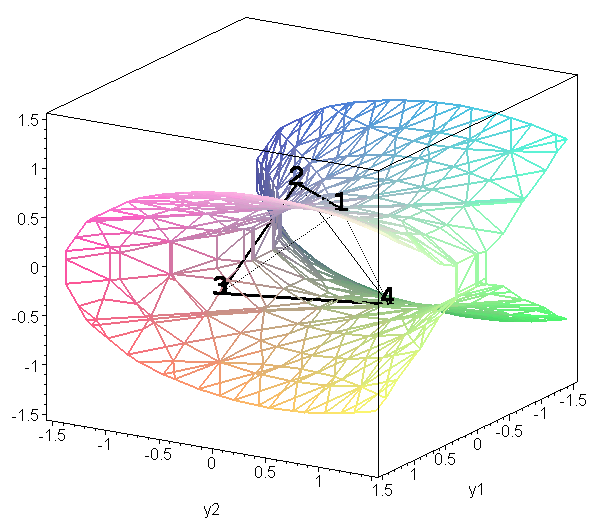
\includegraphics[width=0.9\textwidth]{hyperboloid_p4.png}
\end{center}
\caption{Standard clique wrapper of graph $P_4$}
\end{figure}

The main consequence of the introduced wrapper notion is that we can formulate
now the maximum weight clique problem as a least squares program, that is,
finding a point of some subset of $\mathbb{R}^n$ closest to the origin.

\begin{defn}
The {\em indicator} of a vertex subset $S \subseteq V$ is a point
$x^S \in \mathbb{R}^n$ such that
\[ x^S_i = \left\{ \begin{array}{rl}
  z_i/W(S), & \textrm{if} \ i \in S \\
  0,        & \textrm{if} \ i \in V \setminus S.
\end{array} \right. \]
\end{defn}
It is easy to see that $x^S$ is the orthogonal projection of the origin onto
the face of $\Delta^{(w)}_n$ formed by $S$. So, $x^S$ is the point of this
face closest to the origin. The distance is
\[ \sqrt{\sum_{i \in S} (z_i/W(S))^2} = \sqrt{\sum_{i \in S} w_i/W^2(S)} = 1/\sqrt{W(S)}. \]
Obviously, the heavier a vertex subset, the less the distance to its
indicator and, hence, to the face of $\Delta^{(w)}_n$ it forms. Therefore, we
solve the maximum weight clique problem if we find a common point of
$\Delta^{(w)}_n$ and a clique wrapper closest to the origin.

\begin{thm}
\label{thm:minnorm}
\begin{equation}
\label{eq:minnorm}
1/\omega(G,w) = \min x^T x,
\end{equation}
\[ \mbox{s.t. } x^T H x = 1, \ z^T x = 1, \ x \geq 0, \]
where $H$ is an $n \times n$ real symmetric matrix such that
$h_{ij} = z_i z_j$ if $i=j$ or $(i,j) \in E$ and $h_{ij} < z_i z_j$ otherwise.
The indicator of a maximum weight clique $x^Q$ is a global minimizer of
(\ref{eq:minnorm}).
\end{thm}
{\em Proof.} Follows immediately from the definitions and propositions above.
QED.

\section{The relaxed least squares program}

We will also consider the relaxed version of the program (\ref{eq:minnorm}),
where the nonnegativity constraint $x \geq 0$ is dropped. We can prove that
such a relaxed program is enough to recognize a special type of maximal
cliques.

\begin{thm}
\label{thm:exact}
Let $Q$ be a maximal clique of the graph $G(V,E)$ with the vertex weights $w$
and $H$ be its wrapping matrix. If
\begin{equation}
\label{eq:rsclique}
\forall i \in V \setminus Q \ \sum_{j \in Q} h_{ij} z_j = C z_i,
\end{equation}
where $C$ is a constant, then the indicator of $Q$
\[ x_i = \left\{ \begin{array}{ll}
  z_i/W(Q), & i \in Q \\
  0, & i \in V \setminus Q
\end{array} \right. \]
is a stationary point of the program
\begin{equation}
\label{eq:minnormrelax}
\min x^T x,
\end{equation}
\[ \mbox{s.t. } x \in {\cal W}^H(G,w). \]
\end{thm}
{\em Proof.} Consider the Lagrangian of the program (\ref{eq:minnormrelax})
\begin{displaymath}
L(x,\mu,\eta) = x^T x - \frac{1}{\mu}(x^T H x - 1) + 2 \eta (z^T x - 1)
\end{displaymath}
(we represent here the first Lagrangian multiplier as $-1/\mu$ and the second
one as $2 \eta$ for the sake of convenience.) The stationary points are
those satisfying the system of equations
\[
\frac{1}{2} \frac{\partial L}{\partial x_i} = x_i -\frac{1}{\mu} \sum_{j \in V} h_{ij} x_j + \eta z_i = 0, \ \forall i \in V.
\]
Let $i \in Q$. Then, since $x$ is the indicator of $Q$,
\[
z_i/W(Q) -\frac{1}{\mu} \sum_{j \in Q} \frac{z_i w_j}{W(Q)} + \eta z_i = 0.
\]
Dividing this expression by $z_i$ and reducing the second term, we obtain
\[ 1/W(Q) - 1/\mu + \eta = 0. \]
Now, let $i \in V \setminus Q$. Then we obtain
\[ -\frac{1}{\mu} \sum_{j \in Q} \frac{h_{ij} z_j}{W(Q)} + \eta z_i = 0. \]
If the equality $\sum_{j \in Q} h_{ij} z_j = C z_i$ holds, then it can be
reduced to
\[ -\frac{C}{\mu W(Q)} + \eta = 0. \]
So, the stationary point criterion is reduced to two equations over two
variables, and they are satisfied by
\[ \mu = W(Q)-C, \ \eta = \frac{C}{W(Q)(W(Q)-C)}. \]
Since $Q$ is a maximal clique and $h_{ij} < z_i z_j$ for any $(i,j) \notin E$,
we have $W(Q)>C$. Thus, this solution does not contain a division by $0$.

We have shown that under the imposed condition the indicator of $Q$
satisfies the stationary point criterion with the derived values of Lagrangian
multipliers. QED.

\vspace{1pc}

We mention remarkable corollaries of Theorem \ref{thm:exact}.

\begin{cor}
\label{cor:exact2}
Let $Q$ be a maximal clique of the graph $G(V,E)$ with the vertex weights $w$
such that $\forall i \in V \setminus Q \ W(N(i) \cap Q) = C$, where $C$ is
a constant. Then the indicator of $Q$ is a stationary point of the program
\begin{equation}
\label{eq:minnormrelax2}
\min x^T x,
\end{equation}
\[ \mbox{s.t. } x \in {\cal W}_0(G,w), \]
where ${\cal W}_0(G,w)$ is the standard clique wrapper of $G(V,E)$.
\end{cor}

\begin{cor}
\label{cor:exact3}
Let $Q$ be a maximal clique of the graph $G(V,E)$ such that
$\forall i \in V \setminus Q \ |N(i) \cap Q| = C$, where $C$ is a constant.
Then the unweighted indicator of $Q$
\[ x_i = \left\{ \begin{array}{ll}
  1/|Q|, & i \in Q \\
  0, & i \in V \setminus Q
\end{array} \right. \]
is a stationary point of the program
\begin{equation}
\label{eq:minnormrelax3}
\min x^T x,
\end{equation}
\[ \mbox{s.t. } x^T (A_G+I) x = 1, \ e^T x = 1. \]
\end{cor}

\section{Connection to the Motzkin-Straus theorem and QUALEX-MS algorithm}

In \cite{B02} we established the rescaled Motzkin-Straus formulation for
the maximum weight clique problem very similar in form to Theorem
\ref{thm:minnorm}. We formulate it here again to show the direct connection
between these two formulations.
\begin{prop}[Busygin \cite{B02}]
\label{fact:msagw}
The global optimum value of the quadratic program
\begin{equation}
\label{eq:msagwclique}
\max f(x) = x^T A^{(w)}_G x
\end{equation}
subject to
\begin{equation}
\label{eq:msagwconstr}
z^T x = 1, \; x \geq 0
\end{equation}
is
\[ 1-\frac{w_{\min}}{\omega(w,G)}. \]
Also, there is a global maximizer, where the set of nonzero variables
designates a maximum weight clique and the value of each of those
variables is
\begin{equation}
\label{eq:msagwx}
x_i = \frac{z_i}{\omega(w,G)}.
\end{equation}
\end{prop}
It is easy to see that $A^{(w)}_G=H_0(G,w)-w_{\min}I$. For a clique indicator
$x^Q$ the value of (\ref{eq:msagwclique}) is $1-w_{\min}/W(Q)$. On the other
hand, $(x^Q)^T (w_{\min}I) x^Q = w_{\min}/W(Q)$. So, we may immediately infer
from here the first property of the clique wrapper:
$(x^Q)^T H_0(G,w) x^Q = 1$ for any clique $Q$.

Another remarkable connection is Corollary \ref{cor:exact2} vs. the following
theorem.
\begin{thm}[Busygin \cite{B02}]
\label{thm:exact4}
Let $Q \subseteq V$ be a maximal clique of the graph $G(V,E)$ such that
\[ \forall v \in V \setminus Q: \ W(N(v) \cap Q) = C, \]
where $C$ is some fixed value. Then the indicator $x^Q$ of $Q$
\[ x^Q_i = \left\{ \begin{array}{rl}
  z_i/W(Q), & \textrm{if} \ i \in Q \\
  0,        & \textrm{if} \ i \in V \setminus Q.
\end{array} \right. \]
is a stationary point of the program
\begin{equation}
\label{eq:cliquesphere1}
\max f(x) = x^T A^{(w)}_G x
\end{equation}
\[ \mbox{s.t. } z^T x = 1, \; x^T x \leq r^2, \]
when the parameter $r=1/\sqrt{W(Q)}$.
\end{thm}

\section{How to find the stationary points}

Now we consider finding stationary points of the relaxed program
(\ref{eq:minnormrelax}). First, we move the origin into its orthogonal
projection onto the hyperplane \mbox{$z^T x = 1$}.
\begin{equation}
\label{eq:x0}
x^0=z/W(V).
\end{equation}
That is, we introduce new variables \mbox{$\hat{x} = x - z/W(V)$}. This way
we obtain
\[ \min \hat{x}^T \hat{x} \]
\[ \mbox{s.t. } \hat{x}^T H \hat{x} + 2 (x^0)^T H \hat{x} = s, \ z^T \hat{x} = 0, \]
where $s = 1 - (x^0)^T H x^0$. We note that since $x^0 \in \Delta^{(w)}_n$,
$s \geq 0$ and unless the graph is complete (which would be most trivial for
the clique problem), $s>0$. Now the second constraint determines a linear
subspace. The orthogonal projector onto it is a matrix
$P=(p_{ij})_{n \times n}$, where
\[ p_{ij} = \left\{ \begin{array}{rl}
      1-w_i/W(V), & \textrm{if} \ i=j \\
  - z_i z_j/W(V), & \textrm{if} \ i \neq j.
\end{array} \right. \]
Thus, the program may be reformulated as
\begin{equation}
\label{eq:minnormrelax4}
\min \hat{x}^T \hat{x}
\end{equation}
\[ \mbox{s.t. } \hat{x}^T \hat{H} \hat{x} + 2 \hat{b}^T \hat{x} = s, \]
where $\hat{H}=PHP$ and $\hat{b}^T=(x^0)^T HP$. The only remaining
constraint is a quadratic equality. Diagonalize its quadratic form performing
the eigendecomposition
\[ \hat{H} = Q \textrm{diag}(\lambda_1, \ldots, \lambda_k) Q^T, \]
\[ \lambda_1 \leq \lambda_2 \leq \ldots \leq \lambda_k, \]
and transform its linear form into the new eigenvector basis correspondingly
\[ c = Q^T \hat{b}. \]
Here we consider only eigenvectors whose corresponding eigenvalues and
the linear form coefficients are not zeroes simultaneously. Its number
$k \leq n-1$ because the quadratic form was projected onto an
$(n-1)$-dimensional subspace. So, $Q$ is the $n \times k$ matrix of
eigenvectors (stored as columns.) This way we formulate the program
(\ref{eq:minnormrelax4}) in the eigenvector space
\begin{equation}
\label{eq:minnormrelax5}
\min y^T y,
\end{equation}
\[ \mbox{s.t. } y^T \textrm{diag}(\lambda_1, \ldots, \lambda_k) y + 2 c^T y = s, \ y \in \mathbb{R}^k, \]
where
\[ \hat{x} = Qy, \ y = Q^T \hat{x}. \]
The Lagrangian of (\ref{eq:minnormrelax5}) is
\[ L(y,\mu) = y^T y - \frac{1}{\mu} (y^T \textrm{diag}(\lambda_1, \ldots, \lambda_k) y + 2 c^T y - s). \]
We take the Lagrangian multiplier as $-1/\mu$ for the sake of simplicity
of further expressions. The stationarity criterion
\begin{equation}
\label{eq:stat}
\frac{1}{2} \frac{\partial L}{\partial y_i} = y_i - \frac{1}{\mu} (\lambda_i y_i + c_i) = 0
\end{equation}
gives
\begin{equation}
\label{eq:yi}
y_i = \frac{c_i}{\mu - \lambda_i}.
\end{equation}
Plugging these expressions in the constraint, we obtain a univariate equation
\begin{equation}
\label{eq:secular}
\sum_{i=1}^{k} \frac{c_i^2 (2 \mu - \lambda_i)}{(\mu - \lambda_i)^2} = s.
\end{equation}
Unless there is a degenerate case of multiple eigenvalues with $c_i=0$
corresponding to them, this equation encodes all stationary
points of the program (\ref{eq:secular}). It is equivalent to
a polynomial of degree $2k$, so there are not more than $2k$ stationary
points to consider. First, we address the intervals
$(\lambda_i, \lambda_{i+1})$ where $\lambda_i>0$. Let us prove that
the left-hand side of (\ref{eq:secular}) is unimodal on each of these
intervals. Denote 
\[ f(\mu) = \sum_{i=1}^{k} \frac{c_i^2 (2 \mu - \lambda_i)}{(\mu - \lambda_i)^2}. \]
First of all, notice that
\[ \lim_{\mu \to \lambda_i^+} f(\mu) = +\infty \]
and
\[ \lim_{\mu \to \lambda_{i+1}^-} f(\mu) = +\infty. \]
Then we have
\[ f'(\mu) = \sum_{i=1}^{k} \frac{-2 c_i^2 \mu}{(\mu - \lambda_i)^3} = 2 \mu g(\mu), \]
where
\[ g(\mu) = \sum_{i=1}^{k} \frac{-c_i^2}{(\mu - \lambda_i)^3}. \]
Since $\mu \neq 0$, $f'(\mu)=0$ if and only if $g(\mu)=0$. Differentiating
$g(\mu)$, we obtain
\[ g'(\mu) = \sum_{i=1}^{k} \frac{3 c_i^2}{(\mu - \lambda_i)^4} > 0, \]
which proves that $g(\mu)$ is monotonically increasing on each interval. Now,
since
\[ \lim_{\mu \to \lambda_i^+} g(\mu) = -\infty \]
and
\[ \lim_{\mu \to \lambda_{i+1}^-} g(\mu) = +\infty, \]
$g(\mu)$ must have exactly one root on $(\lambda_i,\lambda_{i+1})$, which we
will denote by $\mu_i^*$. Therefore, $f(\mu)$ is a U-shaped unimodal function
on each interval $(\lambda_i, \lambda_{i+1})$ where $\lambda_i>0$ attaining
the minimum at $\mu_i^*$. If $f(\mu_i^*)<s$, there are two roots, if
$f(\mu_i^*)=s$, $\mu_i^*$ is the only root, and if $f(\mu_i^*)>s$, there are
no roots on $(\lambda_i,\lambda_{i+1})$. Utilizing unimodality of $f(\mu)$,
and boundedness of the interval, it is easy to find $\mu_i^*$ by the golden
section method. Then, if $f(\mu_i^*)<s$, we may use the bisection method to
find a root on $(\lambda_i,\mu_i^*)$ and $(\mu_i^*,\lambda_{i+1})$.

We are also interested in the interval $(\lambda_k, +\infty)$. As
\[ \lim_{\mu \to \lambda_k^+} f(\mu) = +\infty \]
and
\[ \lim_{\mu \to +\infty} f(\mu) = 0 < s, \]
we immediately infer that there is always at least one root on this interval.
Noticing that
\[ f'(\mu) = \sum_{i=1}^{k} \frac{-2 c_i^2 \mu}{(\mu - \lambda_i)^3} < 0 \]
for any $\mu>\lambda_k$, we conclude that there must be exactly one root, which
we will denote by $\mu_k^*$. It is easy to establish an upper bound on it
replacing all $\lambda_i$ in $f(\mu)$ by $\lambda_k$ and solving the equation
for $\mu>\lambda_k$. Indeed,
\[ \frac{\partial}{\partial \lambda_i} \frac{2 \mu - \lambda_i}{(\mu - \lambda_i)^2} = \frac{3 \mu - \lambda_i}{(\mu - \lambda_i)^3} > 0 \]
if $\mu>\lambda_i$, so plugging $\lambda_k$ in $f(\mu)$ instead of every
$\lambda_i$ only increases the expression. Thus,
\[ f(\mu) < \sum_{i=1}^k c_i^2 \frac{2 \mu - \lambda_k}{(\mu - \lambda_k)^2}. \]
Solving a quadratic equation
\[ \sum_{i=1}^k c_i^2 (2 \bar\mu - \lambda_k) = s (\bar\mu - \lambda_k)^2 \]
for $\bar\mu>\lambda_k$ yields the upper bound $\bar\mu$ on $\mu_k^*$. Then,
either the bisection or some Newton-type method can be used to find it.


\begin{thebibliography}{10}

\bibitem{BBPP99}
  I.M. Bomze, M. Budinich, P.M. Pardalos, and M. Pelillo,
  The maximum clique problem,
  in: D.-Z. Du and P.M. Pardalos, eds.,
  {\em Handbook of Combinatorial Optimization\/} (Supplement Volume A),
  Kluwer Academic (1999), 1--74.

\bibitem{B02}
  S. Busygin,
  A New Trust Region Technique for the Maximum Weight Clique Problem,
  {\em Discrete Applied Mathematics 154(15) (International Symposium
  on Combinatorial Optimization CO'02)\/}, pp. 2080--2096, 2006.
  Preprint available at \verb|http://www.stasbusygin.org/writings/qualex-ms.pdf|

\bibitem{GJ79}
  M. Garey and D. Johnson,
  {\em Computers and Intractability: A Guide to the Theory of NP-Completeness\/}
  (Freeman \& Co., 1979).

\bibitem{H96}
  J. H\aa stad,
  Clique is hard to approximate within $n^{1-\epsilon}$,
  in: {\em Proc. 37th Annual IEEE Symposium on the Foundations of
  Computer Science (FOCS)\/} (1996) 627--636.

\bibitem{K01}
  S. Khot,
  Improved inapproximability results for maxclique, chromatic number and
  approximate graph coloring,
  in: {\em Proc. 42nd Annual IEEE Symposium on the Foundations of
  Computer Science (FOCS)\/} (2001) 600--609.

\end{thebibliography}

\end{document}
